\documentclass{beamer}
\DeclareFontShape{OT1}{cmss}{b}{n}{<->ssub * cmss/bx/n}{} 
\usetheme{default}
\usepackage{amsmath}
\usepackage{amsfonts}
\usepackage{mathbbol}
\usepackage{xcolor} % before tikz or tkz-euclide if necessary
\usepackage{tkz-euclide} % no need to load TikZ
\usepackage{multirow}
\usepackage{lmodern}
\usepackage{bm}

\title{Statistical Machine Learning\\ Part 6}
\author{Horacio G\'omez-Acevedo\\ Department of Biomedical Informatics}
\begin{document}
	\begin{frame}[plain]
		\maketitle
	\end{frame}


\begin{frame}{Resampling Methods for Parameter Estimation}
	Suppose you have applied your state of the art algorithm, but you don't know what is the distribution of a parameter (hyperparameter). The question is: how do I determine the bias and variance?
	
	The {\bf jackknife} and {\bf bootstrap} are {\it resampling} methodologies that help improving classification.
	
	
	 
\end{frame}

\begin{frame}{Jacknife}
	It was introducied by Maurice Quenouille around 1950's.  Let's start with an example as motivation for the use of the jacknife. 
	
	{\bf Example. } Let's suppose that we have 
	$m$ independent random variables $X_1,\ldots, X_m$ that follow the same distribution. We can define the statistic $\overline{X}$ defined as $\frac{X_1 + \cdots + X_m}{m}$. The question is what is the standard deviation of this statistic given a set of observed values $X_1=x_1,\ldots, X_m=x_m$?
	
	Following the definition of variance, we can determine
	
	\begin{equation}
		\widehat{\sigma}^2(\overline{X})= \frac{1}{m(m-1)} \sum_{i=1}^m (x_i - \overline{x})^2
		\label{eq:stdev}
	\end{equation}
	
	That was simple enough, but what about calculating an estimate of the variance for other common statistics as  {\it mode}, or {\it median} or other statistics?
	
\end{frame}

\begin{frame}{Jackknife}
	Let's define the sample average of the data set deleting the jth variable as
	\begin{equation*}
		\overline{X}_{(j)}= \frac{1}{m-1} \sum_{k\ne j} X_k
	\end{equation*}
We also define the statistic that is the {\it average} of these averages
\begin{equation*}
	\overline{X}_{(\bullet)} = \frac{1}{m} \sum_{k=1}^m \overline{X}_{(k)}
\end{equation*}

The {\bf Jackknife} estimate of the standard deviation is
\begin{equation}
	\widehat{\sigma}_{Jack}^2(\overline{X})= \frac{m-1}{m} \sum_{i=1}^m (\overline{X}_{(i)} - \overline{X}_{(\bullet)})^2
\label{eq:jstdev}
\end{equation}

It can be verified that (\ref{eq:stdev}) and (\ref{eq:jstdev})  coincide; however, this process allows a generalization of this method.
\end{frame}

\begin{frame}{Jackknife}
	One of the biggest advantages of the expression (\ref{eq:jstdev}) is that when we  have an estimator $\hat{\theta}(x_1,\ldots, x_m)$ of the statistic $\theta$, we can actually estimate the variance of such estimator
	\begin{equation*}
		\hat{\sigma}_{jack}^2= \frac{m-1}{m} \sum_{i=1}^m (\hat{\theta}_{(i)}- \hat{\theta}_{(\bullet)})^2,
	\end{equation*}
where
\begin{equation*}
	\begin{split}
		\hat{\theta}_{(i)}&= \hat{\theta}(x_1, \ldots, x_{i-1},x_{i+1},\ldots, x_m) \\
		\hat{\theta}_{(\bullet)}&= \frac{1}{m-1} \sum_{i=1}^n \hat{\theta}_{(i)} 
	\end{split}
\end{equation*}

\end{frame}
		
\begin{frame}{Jackknife bias}
	It is also possible to obtain the {\bf jackknife bias} estimation
	
	Recall the definition of bias
	\begin{equation*}
		bias = \theta - E(\hat{\theta})
	\end{equation*} 
The Jackknife estimate of bias is given by

\begin{equation*}
	bias_{jack}= (m-1) (\hat{\theta}_{(\bullet)}- \hat{\theta})
\end{equation*}
\end{frame}		
		
\begin{frame}{Bootstrap}
	In a common definition, a {\it bootstrap} data set is one created by randomly selecting $m$ points (with replacement) from the training set $\cal{D}$.
	
	For example if our training data set consists of the points $\{(x_1,y_1),(x_2,y_2),(x_3,y_3)\}$, then a bootstrap could be 
	
	\begin{equation*}
		\begin{split}
				B_1&=\{(x_1,y_1),(x_2,y_2),(x_3,y_3)\}\\
				B_2&=\{(x_1,y_1),(x_1,y_1),(x_2,y_2)\} \\
				B_3&=\{(x_2,y_2),(x_3,y_3),(x_2,y_2)\} 
		\end{split}
	\end{equation*}
	 
\end{frame}		

\begin{frame}{Bootstrap}
	
	The bootstrap was developed by Bradley Efron in the late 1970s. 
	
	In the bootstrap setup, the data sets (say $B_j$s in our example) are treated as independent sets. The {\bf bootstrap} estimate of a statistic $\theta$ is defined as
	
	\begin{equation*}
		\hat{\theta}^{*(\bullet)}= \frac{1}{B} \sum_{b=1}^B \hat{\theta}^{*(b)},
	\end{equation*}
where $\hat{\theta}^{*(b)}$ is the estimate of $\theta$ for the sample $b$ .
\end{frame}		

\begin{frame}{Bootstrap bias and variance estimates}
	The bootstrap estimate of the bias 
	\begin{equation*}
		bias_{boot}= \hat{\theta}^{*(\bullet)}- \hat{\theta}
	\end{equation*}
	Whereas the bootstrap estimate of the variance is
	\begin{equation*}
		\hat{\sigma}^2 (\theta)= \frac{1}{B}\sum_{b=1}^B \left(  \hat{\theta}^{*(b)} - \hat{\theta}^{*(\bullet)} 
		\right)
	\end{equation*}
\end{frame}

\begin{frame}{Subset Selection (Regression)}
	We have seen than when several predictors are present, it is difficult to determine which ones to keep or discard. 
	
	There are some alternatives:
	\begin{itemize}
		\item Best Subset Selection
		\item Stepwise Selection
		\begin{itemize}
			\item Forward Selection
			\item Backwards Selection
		\end{itemize}
	\end{itemize}
\end{frame}

\begin{frame}{Best Subset Selection (Regression) }
	
	Let's suppose we have a linear regression model
	\begin{equation*}
		Y = \theta_0+ \theta_1 X_1 + \cdots + \theta_p X_p + \varepsilon
	\end{equation*}
In theory, we can make (loads) of models 
\begin{equation*}
	\begin{split}
		{\cal M}_0 &: \hat{Y}= \hat{\theta}_0\\
				{\cal M}_1 &: \hat{Y}= \hat{\theta}_0+ \hat{\theta}_1 X_1 \\
				\vdots&\\
				{\cal M}_p &: \hat{Y}= \hat{\theta}_0+ \hat{\theta}_1 X_1 \\
				{\cal M}_{p+1} &: \hat{Y}= \hat{\theta}+ \hat{\theta_1} X_1+ \hat{\theta}_2 X_2  \\
				\vdots &\\
				{\cal M}_{2^p-1}& \colon \hat{Y }= \hat{\theta}_0+ \hat{\theta}_1 X_1 + \cdots + \hat{\theta}_p X_p 
	\end{split}
\end{equation*}
\end{frame}

\begin{frame}{Best Subset Selection}
	
	Algorithm for Best Subset Selection
	\begin{enumerate}
		\item For $k\in \{1,\ldots,p\}$:
		\begin{enumerate}
			\item Fit all $p \choose k$ models that contain exactly $k$ predictors.
			\item Pick the best among these $p \choose k$ models, and call it $\widehat{\cal M}_k$. The selection is based either by selecting the smallest RSS, or largest $R^2$.
		\end{enumerate}
	\item Select a single best model from among ${\cal M}_0$, $\widehat{\cal M}_1,\ldots, \widehat{\cal M}_p$ using cross-validated prediction error, $C_p$ (AIC), BIC, or adjusted $R^2$.
	\end{enumerate}
Notice that in step 3 we have changed our metric. If we were to proceed with the same metric (say largest $R^2$), we will end up with the model including all parameters since $R^2$ increases monotonically towards 1 as the number of predictors increases. 
\end{frame}

\begin{frame}{Forward Stepwise Selection}
	The algorithm for this problem is stated as
	\begin{enumerate}
		\item For $k=\{0,\ldots, p-1\}$:
		\begin{enumerate}
			\item Consider all $p-k$ models that augment the predictors in $\widehat{\cal M}_k$ with one additional predictor.
			\item Choose the {\it best} among these $p-k$ models and call it $\widehat{\cal M}_{k+1}$. The metric is defined as having the smallest RSS or highest $R^2$.
		\end{enumerate}
	\item Select a single best model from among ${\cal M}_0,\widehat{\cal M}_1,\ldots, \widehat{\cal M}_p$ using corss-validated prediction error $C_p$ (AIC), BIC, or adjusted $R^2$.
		\end{enumerate}
	So, instead of comparing $2^p$ models, we will be comparing $1 + \frac{p(p+1)}{2}$ models. 
	
	Note that the forward stepwise tends to do well in practice, it is not guaranteed to find the best possible model!

\end{frame}

\begin{frame}{Forward Stepwise Selection}
	
	 \begin{figure}[h]
		\centering
		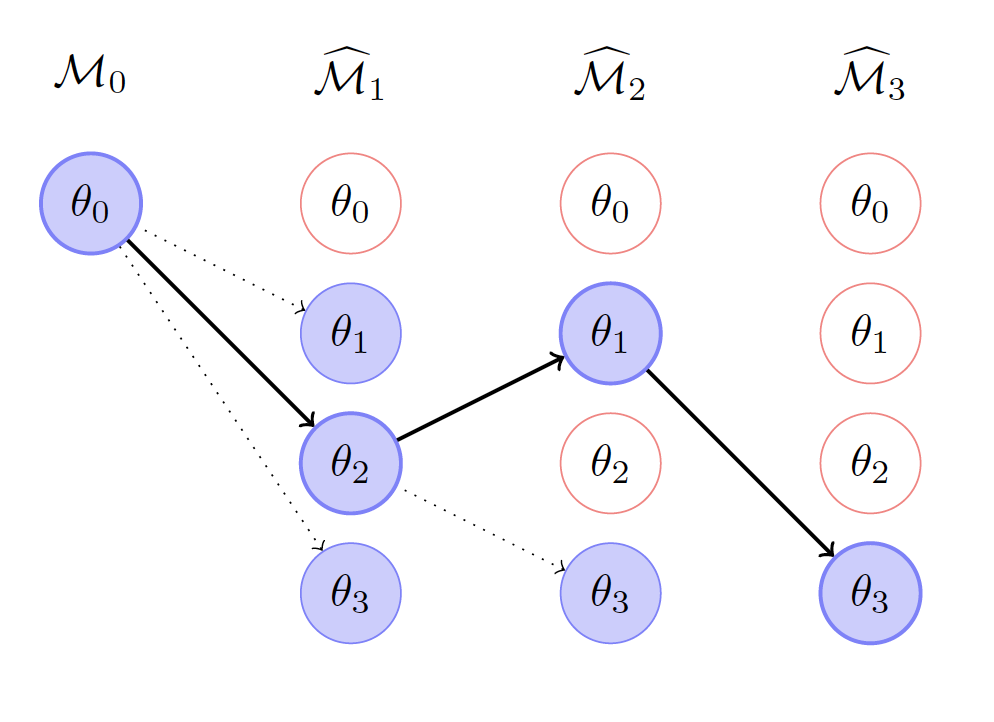
\includegraphics[scale=0.5]{../../Figures/fig_forward.png}
	\end{figure}
\end{frame}

\begin{frame}{Backwards Stepwise Selection}
	It requires the same number of steps as the forward selection. The algorithm runs as follows:
	
	\begin{enumerate}
		\item Let $\widehat{\cal M}_p$  denote the full model with all predictors.
		\item For $k=p,p-1,\ldots,1$:
		\begin{itemize}
			\item Consideer all $k$ models that contain all but one of the predictors in $\widehat{\cal M}_k$, for a total of $k-1$ predictors.
			\item Choose the {\it best} among these $k$ models, and call it $\widehat{\cal M}_{k-1}$. Again, we consider one of the metrics such as the smallest RSS or largest $R^2$.
		\end{itemize}
	 \item Select a single best model from among ${\cal M}_0,\widehat{\cal M}_1, \ldots, \widehat{\cal M}_p$ using cross-validated prediction error, $C_p$ (AIC), BIC or adjusted $R^2$.
	\end{enumerate}
\end{frame}

\begin{frame}{Selection criteria}
	Let's suppose we have fitted a model containing $d$ predictor, the $C_p$ estimate of test MSE is computed using the equation
	\begin{equation*}
		C_p= \frac{1}{n} (RSS+ 2d \hat{\sigma}^2),
	\end{equation*}
	where $\hat{\sigma}^2$ is an estimate of the variance of the error $\varepsilon$ associated with each response measurement. $C_p$ is an unbiased estimate of test MSE. Thus, we choose the model with the lowest $C_p$ value. 
	
	The Akaike information criteria (AIC) is defined for a large class of models fit by maximum likelihood. 
	\begin{equation*}
		AIC \approx \frac{1}{n \hat{\sigma}^2} (RSS+ 2d \hat{\sigma}^2)
	\end{equation*}
 The Bayesian information criteria (BIC) is derived from a Bayesian point of view
 \begin{equation*}
 	BIC \approx \frac{1}{n} (RSS+ \log(n)d \hat{\sigma}^2)
 \end{equation*}

\end{frame}

\begin{frame}{Adjusted $R^2$}
	Finally, the so-called {\bf adjusted} $R^2$ statistic is defined as
	\begin{equation*}
		\textrm{Adjusted }R^2= 1 - \frac{RSS/(n-d-1)}{TSS/(n-1)}= 1 - \frac{n-1}{n-d-1} \cdot \frac{RSS}{TSS}
	\end{equation*}
Recall that $R^2= 1 - RSS/TSS$ where $TSS= \sum (y_i - \overline{y})^2$ is the total sum of squares. 
 So adding the adjusted $R^2$ statistic pays a price for the inclusion of unnecessary variables in the model. 

\end{frame}

\begin{frame}{Optimal Selection}
	
	
 \begin{figure}[h]
	\centering
	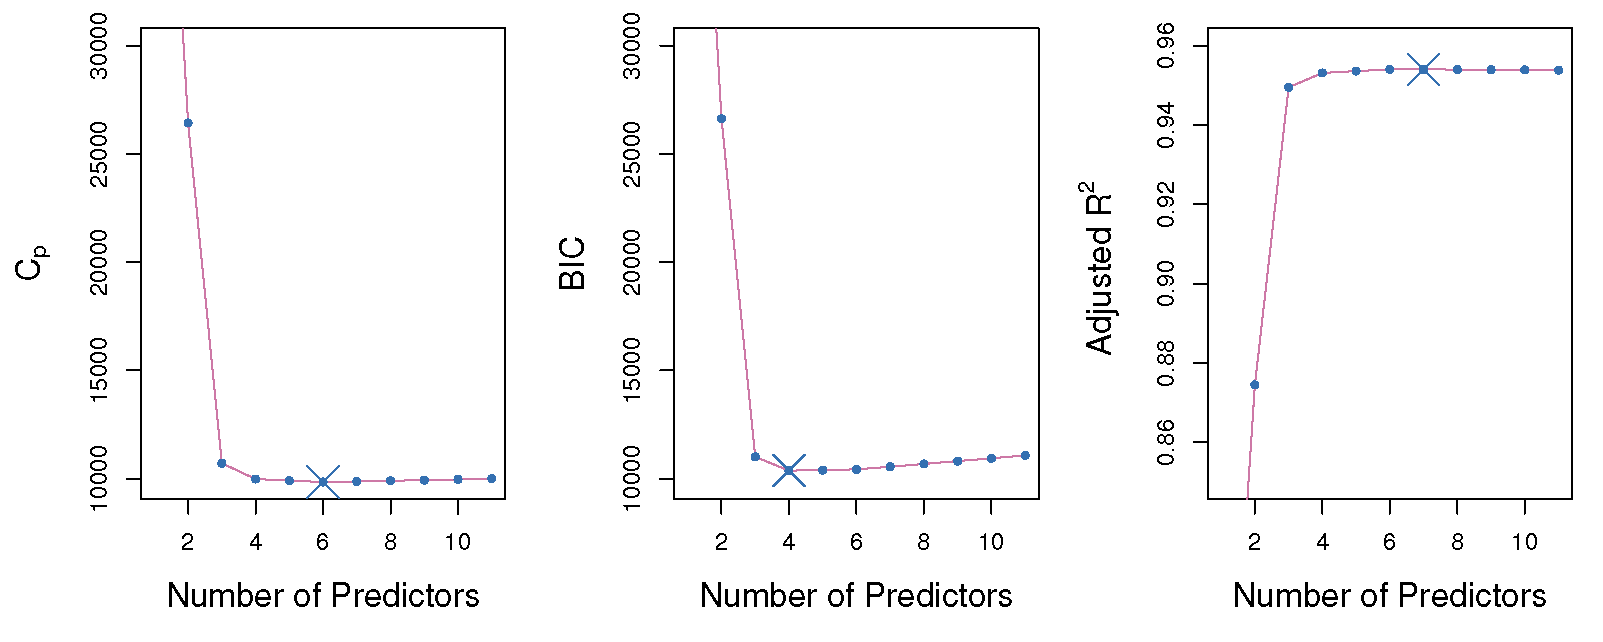
\includegraphics[scale=0.5]{../../Figures/fig_cp.png}
\end{figure}
\end{frame}


\begin{frame}{Final Thoughts}
	
	
	\begin{figure}[h]
		\centering
		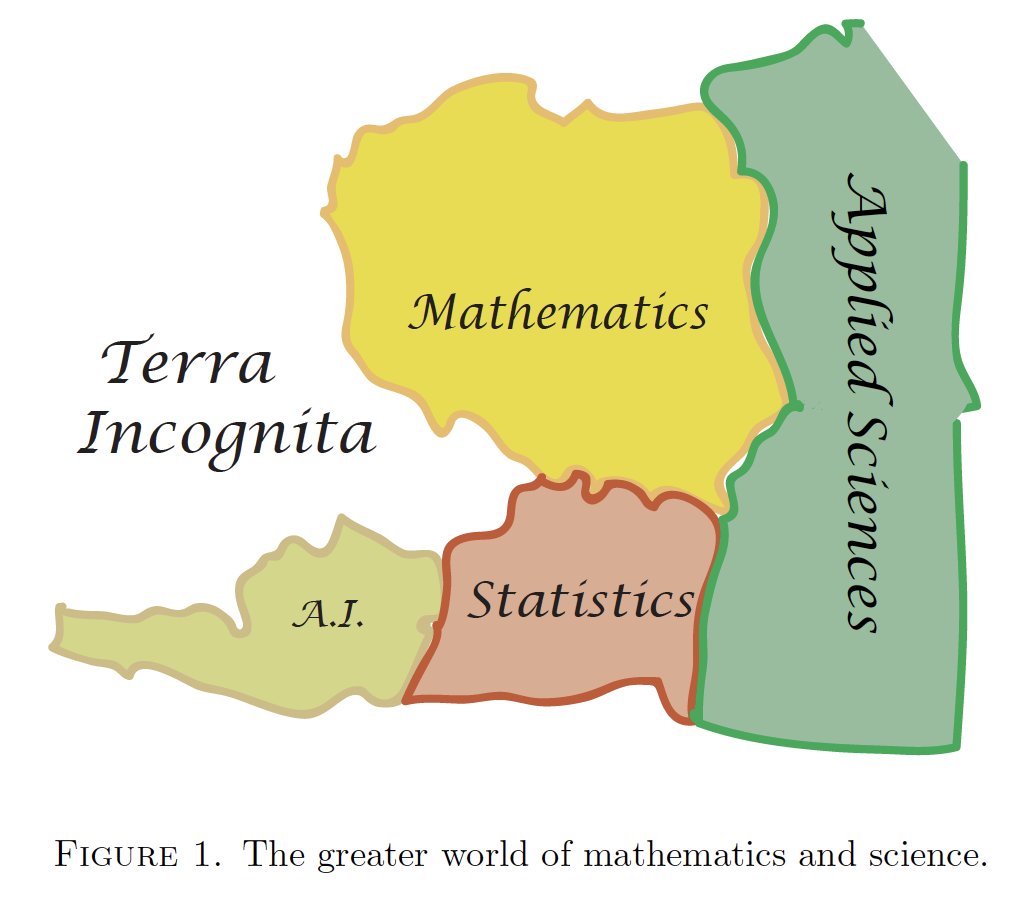
\includegraphics[scale=0.5]{../../Figures/fig_efron_paper.png}
	\end{figure}
\end{frame}
		
	\begin{frame}{References}
		
		Materials and some of the pictures are from (1),(2), and (3).
		\begin{enumerate}
			\item Gareth James et al. {\it An Introduction to Statistical Learning with applications in R}. Springer (2015)
			\item Richard O. Duda et al. {\it Pattern Classification} John Wiley (2001). 
			\item Aur\'elien G\'eron. {\it Hands-on Machine Learning with Scikit-Learn \& TensorFlow} O'Relly (2017)
			\item Wiebe R. Pestman {\it Mathematical Statistics} de Gruyter (1998)
			\item Bradley Efron. {\it The Jackknife, the Bootstrap and other Resampling Plans}  SIAM (1982)
			\item Bradley Efron {\it A 250-year argument: Belief, behavior and the bootstrap} Bull. Am. Math. Soc (2012)
		\end{enumerate}	
		
		I have used some of the graphs by hacking TiKz code from StakExchange, Inkscape for more aesthetic plots and other old tricks of \TeX
	\end{frame}	

	
\end{document}